\documentclass[../main.tex]{subfiles}
\tikzstyle{container} = [draw, rectangle, inner sep=0.3cm]
\begin{document}
\section{Database}
A database is defined as a collection of data and the organization given to this data. The data is organized in tables, in which the data has no formatting. The main difference between a database and a simple spreadsheet is not only the lack of formatting in the database tables, but most importantly the presence of relation that define a structure between the database tables.\\
Data is related using common key (common fields) or common concepts. The use of a structure allow the database tables to be light, in the sense that each table can rely on another one and therefor avoid storing duplicated data allowing for scalability but also for a easiness in the way data is retrieved. 

\begin{figure}[H]
    \centering
\begin{tikzpicture}[scale=0.5, table/.style={matrix of nodes, nodes in empty cells, column sep=-\pgflinewidth, row sep=-\pgflinewidth, nodes={draw,anchor=center,minimum width=2.5cm,minimum height=1cm}, row 1/.style={nodes={minimum height=1cm}}}]
\matrix(User) [table, label=above:Users] {
    \textbf{ID} & \textbf{Name} & \textbf{Surname} \\ 1 & Mario & Rossi \\ 2 & Frank & Weber \\};
\matrix(Time worked) [table, label=above:Time table, right=1cm of User] {
    \textbf{ID} & \textbf{Time [h]} \\ 1 & 4 \\ 2 & 6 \\ 1 & 3 \\ 2 & 8 \\ 2 & 9 \\};
\draw (User-3-1.south)--++(0,-3.5)-|(Time worked-6-1);
\end{tikzpicture}
    \caption{Database Example}
    \label{fig:dbexample}
\end{figure}
\begin{figure}[H]
\begin{center}
\begin{tabular}{ | m{2.5cm} | m{2.5cm}| c | } 
\hline
\textbf{Name} & \textbf{Surname} & \textbf{Time [h]} \\ 
\hline
Mario & Rossi & 4 \\
\hline
Frank & Weber & 6 \\
\hline
Mario & Rossi & 3 \\
\hline
Frank & Weber & 8 \\
\hline
Frank & Weber & 9 \\
\hline
\end{tabular}
\end{center}
    \caption{Spreadsheet like organization}
    \label{fig:spreadsheet}
\end{figure}
In order to better visualize the actual effectiveness of a database an example is presented. The same data is reported in a database like manner in Figure \ref{fig:dbexample} and in a spreadsheet like manner in Figure \ref{fig:spreadsheet}. At first sight, the spreadsheet seems to have less data, indeed no ID is presents making the visualization cleaner. The example is basic and the lack of high volume data makes it hard for the database structure to effectively pop out in its effectiveness. Consider now that all the cells require the same storage capacity in terms of memory (i.e. string and integers require the same memory space), the function governing the number of total cells is for the example reported in Figure \ref{fig:dbexample}, so for the database:
\begin{equation}
    tot = time_{entries} \cdot 2 + ID_{unique} \cdot 3
\end{equation}
While for the case reported in Figure \ref{fig:spreadsheet}, so the spreadsheet:
\begin{equation}
    tot = time_{entries} \cdot 3
\end{equation}
\begin{figure}[H]
    \centering
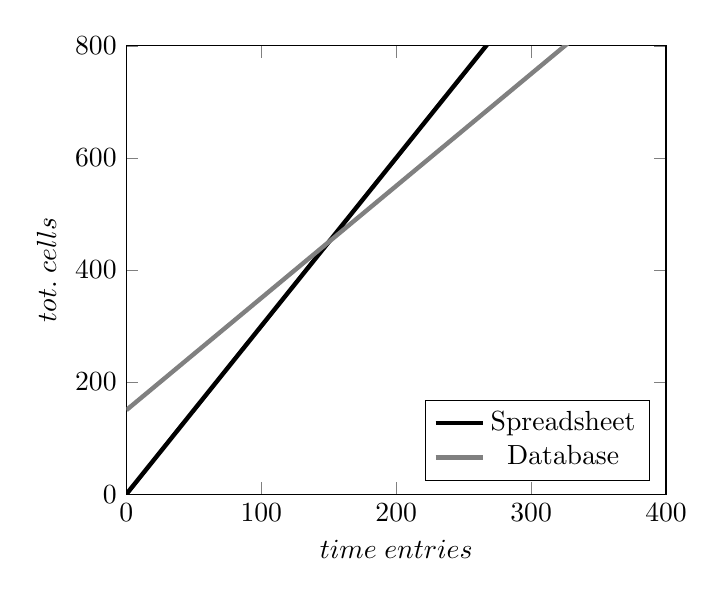
\begin{tikzpicture}[]
\begin{axis}[xmin=0, ymin=0, xmax=400, ymax=800, samples= 100, xlabel=$time\;entries$,ylabel=$tot.\;cells$, legend pos=south east]
  \addplot[black, ultra thick, domain=0:1000] (x,3*x);
  \addplot[gray,  ultra thick, domain=0:1000] (x,2*x + 3*50);
  \addlegendentry{Spreadsheet}
  \addlegendentry{Database}
\end{axis}
\end{tikzpicture}
    \caption{Comparison with 50 User}
    \label{fig:my_label}
\end{figure}
It is easy from the plot, that consider a fixed number of 50 Users that the structured database solution becomes the most effective once the data increases. This is also most efficient when a single entry is comprised by more instances, not only two as in this example case (Name, Surname). A structured database bring others benefits to the picture, such as:
\begin{itemize}
    \item Data accessibility and speed, database integrate querying functionality that can retrieve data based on certain criteria, perform aggregate and calculation across multiple different tables. Other than that the access mechanism is faster than the spreadsheet one, related to the way database data is saved in the memory. 
    \item Data Integrity, in database strict rules are defined for the tables in order to ensure that at the data is accurate and accessible. Relationship between data (ID in Figure \ref{fig:dbexample}) and other matching mechanism as primary keys are part of what is defined Referential Integrity.
    \item Redundancy avoidance, in database, as can be grasped for the example the structure allows for a reduction of redundancy. Duplicates in data mean lack of structure and higher memory consumption. 
    \item Accessibility, database are meant to be worked on by multiple people in a concurrent manner, differently from spreadsheets. This mean a structured user hierarchy is determined in the database. 
\end{itemize}

\subsection{Relational database Management systems}
The previously presented data structure is the one of a type of database defined \textit{Relational Database}. This family of databases uses a user defined structure that allows to identify and access data in relation to another piece of data in the database. Often, data in a relational database is organized into tables.\\ A \gls{RDMS}, Relational Database Management System is used to organize, structure and maintain relational database that are based on the relational model. \gls{SQL} is the language used for handling relational database. \gls{SQL} query language is based on rational algebra and provide an internally consistent mathematical language that makes it easier to improve the performance of all database queries, i.e. data requests from database.
\subsection{User, Roles, Schemas}
Inside a \gls{RDMS} the organization structure, and mostly the access capabilities to the various database instances and table is controlled in by three different level. Schemas, roles and users, this hierarchy is organized as follows:
\begin{itemize}
    \item Roles, roles can be defined on a server basis or on a database basis. A role is a privilege assigned to a certain user. \gls{SQL} defines different standard roles, in order to arbitrate a database. An example can be \texttt{db\char`_owner}, all users assigned this role can perform all configuration and maintenance activities on the database. \texttt{db\char`_datareader} is the role in which users can read data from all user tables. 
    \item Users, a user allow to log in a SQL Server database instance and is mapped to a Login. The main difference between a Login and a User is that a User grant access to a database while Login grant access to a Server. That is the reason why at first a Login need to be created an then a certain User need to be mapped to the respective Login in order to grant the access to both the Server and then the Database
    \item Schema, Schema can be thought as container object that can range from tables, procedures and views. User that are part of a schema can be assigned roles that are valid just for the items in the schema. Therefor they are automatically granted the respective access right to every item that is associated with the schema. An user can have access to just one schema, thus allowing just to access certain object. When creating a new table for example, this just need to be assigned to a certain schema in order to be seen by the user in the schema, without inserting each user singularly. 
\end{itemize}
\subsubsection{Tables}
The data in \gls{RDMS} is stored in objects called tables. A tables, as the on reported in Figure \ref{fig:dbexample} is a collection of related data entries organized in rows and columns.\\
Tables are composed by fields and record. Field in \gls{SQL} language is synonym of column and is designed to maintain specific information about every record in the table. Record refer to a row of data, defined by the sum of the different fields.
\subsubsection{Primary key and foreign key}
The capabilities of creating relations between tables is the basic concept behind relational databases. In order to effectively create data relations the database integrity need to be maintained each time data is added. To ensure that data has no duplicates a mechanism used in SQL is the creation of keys. There are mainly two types of key, primary keys and foreign keys.\\
Each tables that qualify as a relational tables must have a primary key. The primary key consist of one or more columns whose data contained within is used to uniquely identify each row in the table. A primary key can be though as a memory address, it uniquely identify a location, in which data is stored. The relation between tables does not only pass from primary keys. In the \gls{RDMS} a foreign key is a column or a combination of column that match a primary key in another table. Referring to Figure \ref{fig:dbexample} a primary key is represented by the ID in the \textit{Users} table. The foreign key in this case corresponds to the primary key, because the relation between Users and Time table is done via the \textit{ID} field.
% First read
\subsection{Creation of a connection to database on a server}
the database creation require a storing location for the data. The \gls{RDMS} is the application that stores the database data and executes the SQL commands and queries to manipulate the relational database. Other than that, it also manages and performs all the database operations. In order to have access to a database from all the networked the \gls{TCP/IP} protocol is required. \gls{TCP/IP} (Transmission Control Protocol/Internet Protocol) is a set of protocols developed to allow networked computers to share resources over the network. In order to establish a remote connection to the database instances the protocol require that proper set up of Windows firewall. In order to have  a successful connection a tcp port is assigned to the database in a static manner. 
This allow to connect every computer connected to the network to connect via the tcp protocol to the port, thus allowing to access the database instance. Accessing the database instance does not mean that the computer can access the data. Inside the database access rights are defined, as already reported in the section related to it.



\tikzset{every picture/.style={line width=0.75pt}} %set default line width to 0.75pt        
\begin{figure}
    \centering
\begin{tikzpicture}[x=0.75pt,y=0.75pt,yscale=-0.8,xscale=0.8]
%uncomment if require: \path (0,300); %set diagram left start at 0, and has height of 300

%Image [id:dp6531549605845597] 
\draw (386,154.71) node  {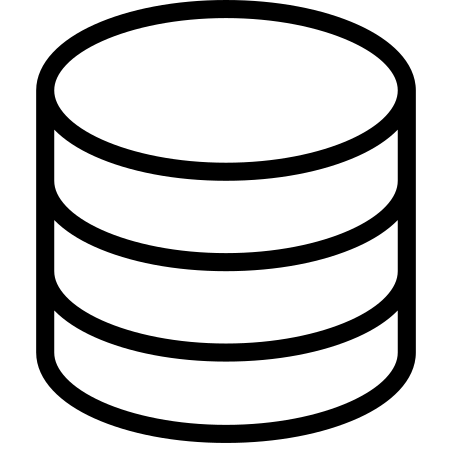
\includegraphics[width=81pt,height=97.93pt]{images_folder/database.png}};
%Image [id:dp05605943116066481] 
\draw (216,156) node  {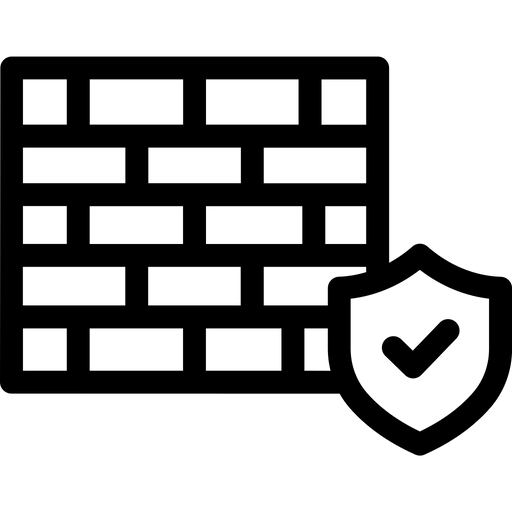
\includegraphics[width=52.5pt,height=52.5pt]{images_folder/firewall-protection-2039809-1721228.png}};
%Image [id:dp383039570021823] 
\draw (64,102.71) node  {
\includegraphics[width=34.5pt,height=35.57pt]{images_folder/pc.png}};
%Image [id:dp5074894649578912] 
\draw (64,163.71) node  {
\includegraphics[width=34.5pt,height=35.57pt]{images_folder/pc.png}};
%Image [id:dp8452106454068984] 
\draw (63,223.71) node  {
\includegraphics[width=34.5pt,height=35.57pt]{images_folder/pc.png}};
%Image [id:dp3665068119749033] 
\draw (595.5,100.21) node  {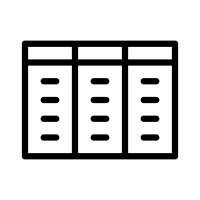
\includegraphics[width=48.75pt,height=51.32pt]{images_folder/935839-200.png}};
%Image [id:dp45105133171160383] 
\draw (595.5,160.21) node  {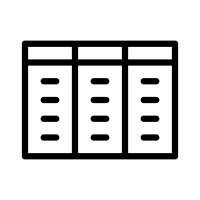
\includegraphics[width=48.75pt,height=51.32pt]{images_folder/935839-200.png}};
%Image [id:dp1763171670611261] 
\draw (595.5,221.21) node  {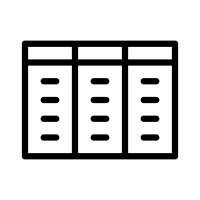
\includegraphics[width=48.75pt,height=51.32pt]{images_folder/935839-200.png}};
%Straight Lines [id:da21693223941443396] 
\draw    (100,101) -- (168.25,139.17) ;
\draw [shift={(170,140.14)}, rotate = 209.21] [color={rgb, 255:red, 0; green, 0; blue, 0 }  ][line width=0.75]    (10.93,-3.29) .. controls (6.95,-1.4) and (3.31,-0.3) .. (0,0) .. controls (3.31,0.3) and (6.95,1.4) .. (10.93,3.29)   ;
%Straight Lines [id:da3176124570414163] 
\draw    (99,220) -- (168.26,181.12) ;
\draw [shift={(170,180.14)}, rotate = 510.69] [color={rgb, 255:red, 0; green, 0; blue, 0 }  ][line width=0.75]    (10.93,-3.29) .. controls (6.95,-1.4) and (3.31,-0.3) .. (0,0) .. controls (3.31,0.3) and (6.95,1.4) .. (10.93,3.29)   ;
%Straight Lines [id:da8563188339305701] 
\draw    (100,159.14) -- (168,160.11) ;
\draw [shift={(170,160.14)}, rotate = 180.82] [color={rgb, 255:red, 0; green, 0; blue, 0 }  ][line width=0.75]    (10.93,-3.29) .. controls (6.95,-1.4) and (3.31,-0.3) .. (0,0) .. controls (3.31,0.3) and (6.95,1.4) .. (10.93,3.29)   ;
%Straight Lines [id:da10650658101917698] 
\draw    (260,160.14) -- (328,161.11) ;
\draw [shift={(330,161.14)}, rotate = 180.82] [color={rgb, 255:red, 0; green, 0; blue, 0 }  ][line width=0.75]    (10.93,-3.29) .. controls (6.95,-1.4) and (3.31,-0.3) .. (0,0) .. controls (3.31,0.3) and (6.95,1.4) .. (10.93,3.29)   ;
%Straight Lines [id:da8525254743123636] 
\draw    (439,120.14) -- (477.19,102) ;
\draw [shift={(479,101.14)}, rotate = 514.5899999999999] [color={rgb, 255:red, 0; green, 0; blue, 0 }  ][line width=0.75]    (10.93,-3.29) .. controls (6.95,-1.4) and (3.31,-0.3) .. (0,0) .. controls (3.31,0.3) and (6.95,1.4) .. (10.93,3.29)   ;
%Straight Lines [id:da9180864032323492] 
\draw    (440,200.14) -- (478.19,218.28) ;
\draw [shift={(480,219.14)}, rotate = 205.41] [color={rgb, 255:red, 0; green, 0; blue, 0 }  ][line width=0.75]    (10.93,-3.29) .. controls (6.95,-1.4) and (3.31,-0.3) .. (0,0) .. controls (3.31,0.3) and (6.95,1.4) .. (10.93,3.29)   ;
%Straight Lines [id:da15194220294106842] 
\draw    (440,161.14) -- (478,161.14) ;
\draw [shift={(480,161.14)}, rotate = 180] [color={rgb, 255:red, 0; green, 0; blue, 0 }  ][line width=0.75]    (10.93,-3.29) .. controls (6.95,-1.4) and (3.31,-0.3) .. (0,0) .. controls (3.31,0.3) and (6.95,1.4) .. (10.93,3.29)   ;
%Straight Lines [id:da09311856378325101] 
\draw    (521,101.14) -- (559,101.14) ;
\draw [shift={(561,101.14)}, rotate = 180] [color={rgb, 255:red, 0; green, 0; blue, 0 }  ][line width=0.75]    (10.93,-3.29) .. controls (6.95,-1.4) and (3.31,-0.3) .. (0,0) .. controls (3.31,0.3) and (6.95,1.4) .. (10.93,3.29)   ;
%Straight Lines [id:da43474826611768935] 
\draw    (521,160.14) -- (559,160.14) ;
\draw [shift={(561,160.14)}, rotate = 180] [color={rgb, 255:red, 0; green, 0; blue, 0 }  ][line width=0.75]    (10.93,-3.29) .. controls (6.95,-1.4) and (3.31,-0.3) .. (0,0) .. controls (3.31,0.3) and (6.95,1.4) .. (10.93,3.29)   ;
%Straight Lines [id:da13431673428420954] 
\draw    (521,221.14) -- (559,221.14) ;
\draw [shift={(561,221.14)}, rotate = 180] [color={rgb, 255:red, 0; green, 0; blue, 0 }  ][line width=0.75]    (10.93,-3.29) .. controls (6.95,-1.4) and (3.31,-0.3) .. (0,0) .. controls (3.31,0.3) and (6.95,1.4) .. (10.93,3.29)   ;
%Image [id:dp9305152591758974] 
\draw (501.14,216.55) node  {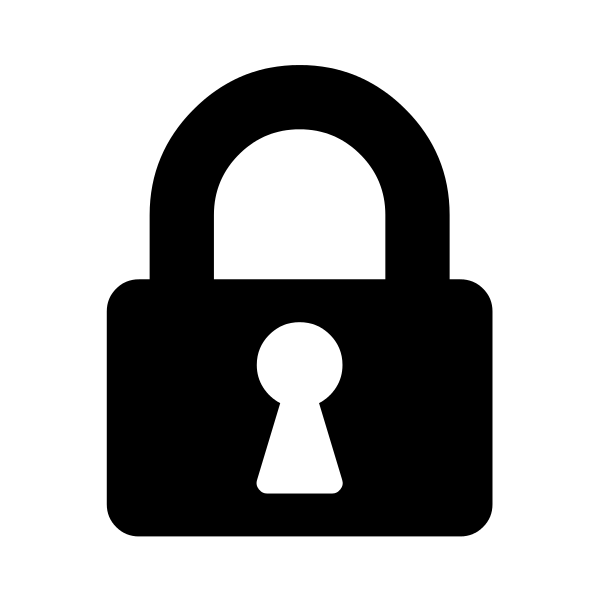
\includegraphics[width=24.22pt,height=26.17pt]{images_folder/lock.png}};
%Image [id:dp22011543040409642] 
\draw (501.14,156.55) node  {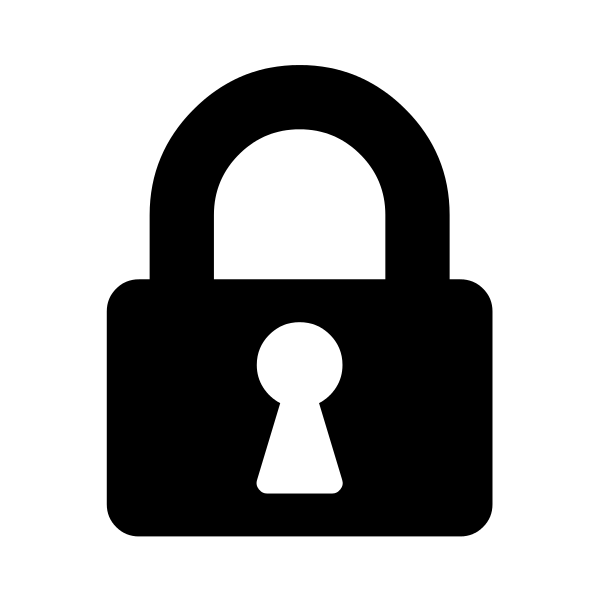
\includegraphics[width=24.22pt,height=26.17pt]{images_folder/lock.png}};
%Image [id:dp43535330126349736] 
\draw (501.14,96.55) node  {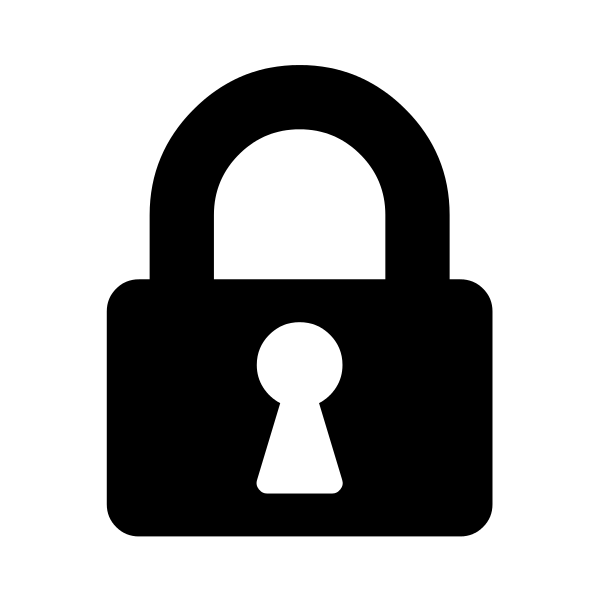
\includegraphics[width=24.22pt,height=26.17pt]{images_folder/lock.png}};

\end{tikzpicture}
    \caption{Database tcp connection schema}
    \label{fig:tcpdb}
\end{figure}

\section{SQLAlchemy}
\label{sec:SQLACHMEYMSEC}
\subsection{Object-relational Mapping}
Object relational mapping is the procedure used to convert between rows in a relational database and object in a programming language \cite{10.1145/1376616.1376773}. The \gls{ORM} sits in between the programmer application and the database and help the programmer abstracting the SQL queries to access, remove and modify the data in the database. 
\subsection{SQL Alchemy working principle}
SQLALchemy is a Python package that develop in order to facilitate the job of creating and maintaining database. Instead of writing SQL queries the developer interface with the database using python. It is not to be forgot that the integration of database management in the python environment allow for flexibility in data storage for a wide range of application that alredy run on python. The organization of the tables is done via Python classes and using then the ORM layer to connect the classes with the tables in the database.\\
SQLAlchemy can be connected to a wide variety of DBMS. To be able to connect the database there is the need of a driver. The function of the driver is the one of translating the SQL queries send by the application to the underlying format the database is using, since in general the database can read different flavours of the SQL language. The scheme of the connection is reported in the following block diagram. 

\tikzstyle{block} = [draw, rectangle, text width=2cm, text centered, minimum height=1.2cm, node distance=3cm]
\begin{figure}[h]
  \centering
\begin{tikzpicture}[scale=0.85,transform shape]
    \node [block, name=text1] {Python class};
    \node [block, right of=text1] (text2) {SQL Alchemy};
    \node [block, right of=text2] (text3) {Driver};
    \node [block, right of=text3] (text4) {Table Object};
    \node [block, right of=text4] (text5) {Database};
    \node [container,fit=(text2) (text3) (text4) ] (container) {};

    \draw [->] (text1) -- (text2);
    \draw [->] (text2) -- node {} (text3);
    \draw [->] (text3) -- node {} (text4);
    \draw [->] (text4) -- node {} (text5);
\end{tikzpicture}
  \caption{ORM layer}
  \label{ormlayer}
\end{figure}
The following example, taken from the SQLAlchemy library showcase how the python code is used to create and update values in a table stored in a database. 

\lstset{language=Python}
\lstset{frame=lines}
\lstset{caption={SQLAlchemy basic example}}
\lstset{label={lst:code_direct}}
\lstset{basicstyle=\footnotesize}
\begin{lstlisting}
from sqlalchemy import create_engine, MetaData, Table, Column, 
Integer, String
from sqlalchemy.ext.declarative import declarative_base

Base = declarative_base()
engine = create_engine('sqlite:///college.db', echo = True)
Session = sessionmaker(bind=engine)

class User(Base):
     __tablename__ = 'users'

     id = Column(Integer, primary_key=True)
     user_name = Column(String)
     user_surname = Column(String)

     def __init__(name, surname):
        user_name = name
        user_surname = surname
        
     def __repr__(self):
        return "<User(name='%s', fullname='%s', nickname='%s')>" % (
                            self.name, self.fullname, self.nickname)
            
# Create the table
Base.metadata.create_all(engine)

#Add new entries
user1 = User("Mario", "Rossi")
Session.add(user1)

user2 = User("Frank", "Weber")
Session.add(user2)

Session.commit()

# Delete entries
Session.delete(user2)
Session.commit()
\end{lstlisting}
Having a flawless interaction between the database and the Python code allow for a better integrated environment. Having a continuous flow of data, originated in the python script and directly, also via the python script send to the database allow for creating a fast updating platform for data analysis. Thanks to the potentiality of the SQL Alchemy library this quest is full filled. 
\section{Database update mechanism}
\cleardoublepage
\end{document}